\chapter{Los conceptos del Cálculo Integral}
\setcounter{chapter}{1}
\setcounter{section}{2}

\section{Funciones. Definición formal como conjunto de pares ordenados}
En cálculo elemental tiene interés considerar en primer lugar, aquellas funciones en las que el dominio y el recorrido son conjuntos de números reales. Estas funciones se llaman 
\textbf{Funciones de variable real} o funciones reales.\\

    \begin{tcolorbox}[colframe=white]
        %-----------------------------1.1. definición par ordenado-----------------------------
        \begin{def.}[Par ordenado]
            Dos pares ordenados $(a,b)$ y $(c,d)$ son iguales si y sólo si sus primeros elementos son iguales y sus segundos elementos son iguales.
            $$(a,b) = (c,d) \; \; \mbox{si y sólo si} \; \; a=c \; y \; b=d$$
        \end{def.}
    \end{tcolorbox}

    \begin{tcolorbox}[colframe=white]
        %----------------------------1.2 definición de función---------------------------------
        \begin{def.}[Definición de función]
            Una función $f$ es un conjunto de pares ordenados $(x,y)$ ninguno de los cuales tiene el mismo primero elemento.\\\\
            Debe cumplir las siguientes condiciones de existencia y unicidad:
            \begin{enumerate}[\bfseries (i)]
                \item $\forall x \in D_f, \exists y / (x,y) \in f(x) \; ó \; y=f(x)$
                \item $(x,y) \in  f \land (x,z) \in  f \Rightarrow y = z$
            \end{enumerate}
        \end{def.}
    \end{tcolorbox}

    \begin{tcolorbox}[colframe=white]
        %----------------------------1.3 definición dominio recorrido---------------------------
        \begin{def.}[Dominio y recorrido]
            Si $f$ es una función, el conjunto de todos los elementos $x$ que aparecen como primeros elementos de pares $(x,y)$ de $f$ se llama el \textbf{dominio} de $f$.  El conjunto de los segundos elementos y se denomina \textbf{recorrido} de $f$, o conjunto de valores de $f$.
        \end{def.}
    \end{tcolorbox}

        %----------------------teorema 1.1------------------------
        \begin{teo}
            Dos funciones $f$ y $g$ son iguales si y sólo si 
            \begin{enumerate}[\bfseries (a)]
                \item $f$ y $g$ tienen el mismo dominio, y
                \item $f(x) = g(x)$ para todo $x$ del dominio de $f.$\\
            \end{enumerate}
            Demostración.- \; Sea $f$ función tal que $x \in  D_f,\exists y \; / \; y=f(x)$ es decir $(x,f(x))$, $g$ una función talque $\forall  z \in  D_g , \exists  y \; / \; y=g(z)$ es decir $(z,g(z))$, entonces por definición de par ordenado tenemos que $(x,f(x)) = (z,g(z)) $ si y sólo si $x=z$ y $f(x)=g(z)$\\\\
        \end{teo}

    \begin{tcolorbox}[colframe=white]
        %--------------1.4 definición de sumas productos y cocientes de una función----------------------
        \begin{def.}[Sumas, productos y cocientes de funciones]
            Sean $f$ y $g$ dos funciones reales que tienen el mismo dominio $D$. Se puede construir nuevas funciones a partir de $f$ y $g$ por adición, multiplicación o división de sus valores. La función $u$ definida por,
            $$u(x) = f(x) + g(x) \; \; si \; x \in D$$
            se denomina suma de $f$ y $g$, se representa por $f+g.$ Del mismo modo, el producto $v=f cdot g$ y el cociente $w=f/g$ están definidos por las fórmulas
            $$v(x) = f(x) g(x) \; \; si \; x \in D, \; \; \, \, w(x) = f(x)/g(x) \; \; si \, x \, \in D \; y \; g(x) \neq 0$$
        \end{def.}
    \end{tcolorbox}
    
\setcounter{section}{4}
\section{Ejercicios}
    \begin{enumerate}[\Large \bfseries 1.]
        %---------------------1.-------------------
        \item Sea $f(x)=x+1$ para todo real $x$. Calcular:
            \begin{itemize}
                \item $f(2) = 2+1 = 3$\\\\
                \item $f(-2) = -2 +1 = -1$\\\\
                \item $-f(2) = -(2+1)=-3$\\\\
                \item $f \left( \dfrac{1}{2} \right) = \dfrac{1}{2} + 1 = \dfrac{3}{2}$\\\\
                \item $\dfrac{1}{f(2)}= \dfrac{1}{3}$\\\\
                \item $f(a+b) = a+b+1$\\\\
                \item $f(a)+f(b)= (a+1) + (b+1) = a+b+2$\\\\
                \item $f(a) \cdot f(b) = (a+1)(b+1) = ab + a + b + 1$\\\\
            \end{itemize}

        %--------------------2.--------------------
        \item Sean $f(x)= 1+x$ \; y \; $g(x)=1-x$ para todo real $x$. calcular:
            \begin{itemize}
                \item $f(2)+g(2) = (1+2) + (1-2) = 2$\\\\
                \item $f(2)-g(2) = (1+2) - (1-2) = 4$\\\\
                \item $f(2)\cdot g(2) = (1+2) \cdot (1-2) = 3 \cdot (-1) = -3$\\\\
                \item $\dfrac{f(2)}{g(2)}= \dfrac{1+2}{1-2} = \dfrac{3}{-1} = -3$\\\\
                \item $f\left[ g(2)\right] = f(1-2) = f(-1) = 1+(-1)= 0$\\\\
                \item $g\left[ f(2)\right] = f(1+2) = g(3) = 1 - 3 = -2$\\\\
                \item $f(a) + g(-a) = (1+a) + (1 - a) = 2$\\\\
                \item $f(t)\cdot g(-t) = (1+t) \cdot (1+t) = 1 + t + t + t^2 = t^2 +2t + 1 = (t+1)^2$\\\\
            \end{itemize}
        
        %--------------------3.---------------------
        \item Sea $f(x)=|x-3|+|x-1|$ para todo real $x$. Calcular:\\
            \begin{itemize}
                \item $f(0) = |0-3|+|0-1| = 3 + 1 = 4$
                \item $f(1) = |1-3|+|1-1| = 2$
                \item $f(2) = |2-3|+|2-1| = -1 + 1 = 2$
                \item $f(3) = |3-3|+|3-1| = 2$
                \item $f(-1) = |-1-3|+|-1-1| = 4 + 2 = 6$
                \item $f(-2) = |-2-3|+|-2-1| = 5 + 3 = 8$\\
            \end{itemize}
            Determinar todos los valores de $t$ para los que $f(t+2)=f(t)$\\
            \begin{center}
                \begin{tabular}{r c l}
                    $|t+2-3| + |t+2-1|$&=&$|t-3| + |t-1|$\\
                    $|t-1|+|t+1|$&=&$|t-3|+|t-1|$\\
                    $|t+1|$&=&$t-3$\\
                \end{tabular}
            \end{center}
            Por lo tanto  $t=1$\\\\


        %--------------------4.-------------------
        \item Sea $f(x)=x^2$  para todo real $x$. Calcular cada una de las fórmulas siguientes. En cada caso precisar los conjuntos de números erales $x, \; y \; t,$ etc., para los que la fórmula dada es válida.
            \begin{enumerate}[\bfseries (a)]
                %----------(a)----------
                \item $f(-x)=f(x)$ \\\\
                Demostración.- \; Se tiene $f(-x) = (-x)^2 = x^2 = f(x) \; \forall x \in \mathbb{R}$\\\\
                %----------(b)----------
                \item $f(y)-f(x)=(y-x)(y+x)$\\\\
                Demostración.- \; $f(y)-f(x)= y^2 - x^2 = (x-y)(x+y), \; \forall x, \; y \in \mathbb{R}$\\\\
                %----------(c)----------
                \item $f(x+h) - f(x) = 2xh + h^2$\\\\
                Demostración.- \; $f(x+h) - f(x) = (x+h)^2 -x^2 = x^2 + 2xh +h^2 - x^2 = 2xh + h^2, \; \forall x \in \mathbb{R}$\\\\
                %----------(d)----------
                \item $f(2y) = 4f(y)$\\\\
                Demostración.- \; $f(2y) = (2y)^2 = 4y^2 = 4 f(y), \; \forall y \in \mathbb{R}$\\\\
                %----------(e)----------
                \item $f(t^2)=f(t)^2$\\\\
                Demostración.- \; $f(t^2) = (t^2)^2 = f(t)^2$\\\\
                %----------(f)----------
                \item $\sqrt{f(a)} = |a|$\\\\
                Demostración.- \; $\sqrt{f(a)} = \sqrt{a^2} = |a|$\\\\
            \end{enumerate}

        %--------------------5.--------------------
        \item Sea $g(x) = \sqrt{4-x^2}$ para $|x| \leq 2$. Comprobar cada una de las fórmulas siguientes e indicar para qué valores de $x, \; y, s$ y $t$ son válidas.
            \begin{enumerate}[\bfseries a)]
                %----------(a)----------
                \item $g(-x) = g(x)$\\\\
                Se tiene $g(-x)=\sqrt{2-(-x)^2} = \sqrt{2-(x)^2} = g(x), \; \; para \; |x| \leq 2$\\\\
                %----------(b)----------
                \item $g(2y) = 2\sqrt{1-y^2}$\\\\
                $g(2y)=\sqrt{4-(2y)^2}= \sqrt{4(1-y^2)} = 2 \sqrt{1-y^2}, \; \; para \; |y|\leq 1$ Se obtiene $|y| \leq 1$  de $\sqrt{1-y^2}$ es decir $1-y^2 \geq 0$ entonces $\sqrt{y^2} \leq \sqrt{1}$ \; y \; $|y|\leq 1$\\\\
                %----------(c)----------
                \item $g\left( \dfrac{1}{t} \right) = \dfrac{\sqrt{4t^2}-1}{|t|}$\\\\
                $g\left( \dfrac{1}{t} \right) = \sqrt{4 - \left( \dfrac{1}{t} \right)^2} = \sqrt{\dfrac{4t^2 - 1}{t^2}} =\dfrac{\sqrt{4t^2 - 1}}{|t|}, \; \; para \; |t| \geq \dfrac{1}{2}$\\\\
                Para hallar los valores correspondientes debemos analizar $\sqrt{4t^2 - 1}$\\\\
                %----------(d)----------
                \item $g(a-2) = \sqrt{4a-a^2}$\\\\
                $g(a-2) = \sqrt{4 - x^2} = \sqrt{4 - (a-2)^2} = \sqrt{4a - a^2}, \; \; para \; 0\leq a \leq 4$\\\\
                %----------(e)----------
                \item $g \left( \dfrac{s}{2} \right) = \dfrac{1}{2} \sqrt{16 - s^2}$\\\\
                $s\left( \dfrac{s}{2} \right) = \sqrt{4 - \left( \dfrac{s}{2} \right)^2} = \dfrac{\sqrt{16 - s^2}}{2}, \; \; para \; |s| \leq 4$\\\\
                %----------(f)----------
                \item $\dfrac{1}{2 +g(x)} = \dfrac{2-g(x)}{x^2}$\\\\ 
                $\dfrac{1}{2 +g(x)} = \dfrac{1}{2+ \sqrt{4-x^2}} \cdot \dfrac{2 - \sqrt{4-x^2}}{2 - \sqrt{4-x^2}} = \dfrac{2 - g(x)}{x^2}\; para \; \; 0 < |x| \leq 2 $\\\\ 
                Evaluemos $\sqrt{4-x^2}$. Sea $4-x^2 \geq 0$ entonce $\sqrt{x^2} \leq 2$. Por otro lado tenemos que la función no puede ser $0$ por $\dfrac{1}{x^2}$, por lo tanto debe ser $x^2\leq 0$.\\\\ 
            \end{enumerate}

        %--------------------6.-------------------
        \item Sea $f$ la función definida como sigue: $f(x)=1$ para $0 \leq x \leq 1;$ $f(x)=2$ para $1 < x \leq 2$. La función no está definida si $x<0$ ó si $x >2.$
            \begin{enumerate}[\bfseries (a)]
                %----------(a)----------
                \item Trazar la gráfica de $f$ 
                    \begin{center}
                        \begin{tikzpicture}[scale=1,draw opacity = 0.6]
                            % abscisa y ordenada
                            \tkzInit[xmax= 3,xmin=0,ymax=3,ymin=0]
                            \tiny\tkzLabelXY[opacity=0.6,step=1, orig=false]
                            % etiqueta x, f(x)
                            \tkzDrawX[opacity=0.6,label=x,right=0.3]
                            \tkzDrawY[opacity=0.6,label=f(x),below = -0.6]
                            %dominio y función
                            \draw [domain=0:1,thick,gray] plot(\x,{1});
                            \tkzText[opacity=0.6,above](0.5,1){\tiny $f(x)=1$}
                            \draw [domain=1:2,thick,gray] plot(\x,{2});
                            \tkzText[opacity=0.6,above](1.5,2){\tiny $f(x)=2$}
                            % intervalos
                            \draw[fill=black] (0,1) circle (1.5pt);
                            \draw[fill=black] (1,1) circle (1.5pt);
                            \draw[          ] (1,2) circle (1.5pt);
                            \draw[fill=black] (2,2) circle (1.5pt);
                        \end{tikzpicture}
                    \end{center}
                %----------(b)----------
                \item Poner $g(x) = f(2x).$ Describir el dominio de $g$ y dibujar su gráfica.
                    \begin{center}
                        \begin{tikzpicture}[scale=1,draw opacity = 0.6]
                            % abscisa y ordenada
                            \tkzInit[xmax= 3,xmin=0,ymax=3,ymin=0]
                            \tiny\tkzLabelXY[opacity=0.6,step=1, orig=false]
                            % label x, f(x)
                            \tkzDrawX[opacity=0.6,label=x,right=0.3]
                            \tkzDrawY[opacity=0.6,label=f(x),below = -0.6]
                            %dominio y función
                            \tkzFct[opacity=1,domain = 0:0.5]{1}
                            \draw [domain=0:0.5,thick,gray] plot(\x,{1}); 
                            \tkzFct[opacity=1,domain = 0.5:1]{2} 
                            % intervalos
                            \tkzSetUpPoint[shape=circle, size = 3, color=black, fill=black]
                            \tkzDefPointByFct[draw,with = a](0)
                            \tkzDefPointByFct[draw,with = a](0.5)
                            \tkzDefPointByFct[draw,with = b](1)
                            \tkzSetUpPoint[shape=circle, size = 3, color=black, fill=white]
                            \tkzDefPointByFct[draw,with = b](0.5)
                        \end{tikzpicture}
                    \end{center}
                Debido a que $1\leq 2x \leq 1$ \; y \; $1 < 2x \leq 2$ el dominio de $g(x)$ es $0\leq x \leq 1$\\\\ 
                %----------(c)----------
                \item Poner $h(x) = f(x-2).$ Describir el dominio de $k$ \; y dibujar su gráfica.
                    \begin{center}
                        \begin{tikzpicture}[scale=1,draw opacity = 0.6]
                            % abscisa y ordenada
                            \tkzInit[xmax= 4,xmin=0,ymax=3,ymin=0]
                            \tiny\tkzLabelXY[opacity=0.6,step=1, orig=false]
                            % label x, f(x)
                            \tkzDrawX[opacity=0.6,label=x,right=0.3]
                            \tkzDrawY[opacity=0.6,label=f(x),below = -0.6]
                            %dominio y función
                            \tkzFct[opacity=1,domain = 2:3]{1} 
                            \tkzFct[opacity=1,domain = 3:4]{2} 
                            % intervalos
                            \tkzSetUpPoint[shape=circle, size = 3, color=black, fill=black]
                            \tkzDefPointByFct[draw,with = a](2)
                            \tkzDefPointByFct[draw,with = a](3)
                            \tkzDefPointByFct[draw,with = b](4)
                            \tkzSetUpPoint[shape=circle, size = 3, color=black, fill=white]
                            \tkzDefPointByFct[draw,with = b](3)
                        \end{tikzpicture}
                    \end{center}
                Debido a que $1\leq x-2 \leq 1$ \; y \; $1 < x-2 \leq 2$ el dominio de $h(x)$ es $2\leq x \leq 4$\\\\ 
                %----------(d)----------
                \item Poner $k(x) = f(2x) + f(x-2).$ Describir el dominio de $k$ \; y dibujar su gráfica.\\\\
                El dominio está vacío ya $f(2x)$ que solo está definido para $0 \leq x \leq 1$ \; y \;  $f(x-2)$ solo está definido para $2 \leq x \leq 4$. Por lo tanto no hay ninguno $x$ que satisfaga ambas condiciones. \\\\
            \end{enumerate}
        
        %--------------------7.-------------------
        \item Las gráficas de los dos polinomios $g(x)=x$ \; y \; $f(x)=x^3$ se cortan en tres puntos. Dibujar una parte suficiente de sus gráficas para ver cómo se cortan.
            \begin{center}
                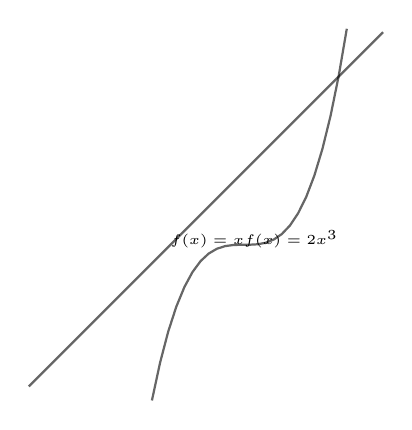
\begin{tikzpicture}[scale=0.9, draw opacity = .6]
                    % abscisa y ordenada
                    \tkzInit[xmax= 3,xmin=-2,ymax=3,ymin=-2]
                    \tiny\tkzLabelXY[opacity=0.6,step=1, orig=false]
                    % label x, f(x)
                    \tkzDrawX[opacity= .6,label=x,right=0.3]
                    \tkzDrawY[opacity= .6,label=f(x),below = -0.6]
                    %dominio y función
                    \draw [domain=-2:3,thick] plot(\x,{\x}); 
                    \tkzText[above,opacity=0.6](3.3,3){\tiny $f(x)=x$}
                    \draw [domain=-1.3:1.45,thick] plot(\x,{\x^3}); 
                    \tkzText[above,opacity=0.6](1.2,3){\tiny $f(x)=2x^3$}
                \end{tikzpicture}
            \end{center}  

        %--------------------8.-------------------
        \item Las gráficas de los dos polinomios cuadráticos $f(x) = x^2-2$ \; y \; $g(x)=2x^2+4x+1$ se cortan en dos puntos. Dibujar las porciones de sus gráficas comprendidas entre sus intersecciones.
            \begin{center}
                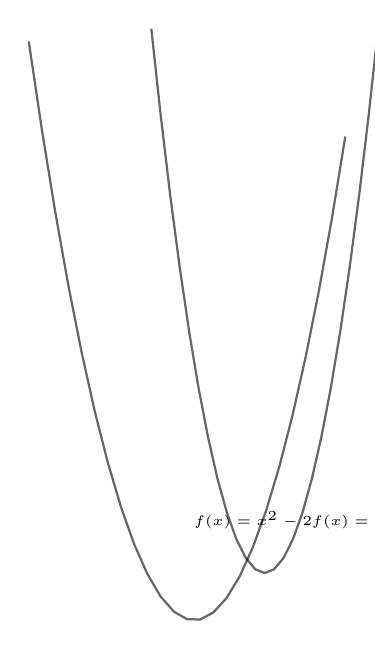
\begin{tikzpicture}[scale=.6, draw opacity = .6]
                    % abscisa y ordenada
                    \tkzInit[xmax= 4,xmin=-4,ymax=10,ymin=-3]
                    \tiny\tkzLabelXY[opacity=0.6,step=1, orig=false]
                    % label x, f(x)
                    \tkzDrawX[opacity= .6,label=x,right=0.3]
                    \tkzDrawY[opacity= .6,label=f(x),below = -0.6]
                    %dominio y función
                    \draw [domain=-3.5:3.2,thick] plot(\x,{\x*\x - 2});  
                    \tkzText[above,opacity=0.6](4,8.2){\tiny $f(x)=x^2 - 2$}
                    \draw [domain=-3.4:1.4,thick] plot(\x,{2*\x*\x + 4*\x + 1});  
                    \tkzText[above,opacity=0.6](3,10.5){\tiny $f(x)=2x^2 +4x + 1$}
                \end{tikzpicture}
            \end{center} 

        %--------------------9.-------------------
        \item Este ejercicio desarrolla ciertas propiedades fundamentales de los polinomios. Sea $f(x)=\displaystyle\sum_{k=0}^{n} c_k x^k$ un polinomio de grado $n$. Demostrar cada uno de los siguientes apartados:
            \begin{enumerate}[\bfseries (a)]
                %----------(a)----------
                \item Si $n \geq 1$ \; y \; $f(0)=0,$ $f(x)=xg(x)$, siendo $g$ un polinomio de grado $n-1.$\\\\
                Para entender lo que nos quiere decir Apostol pongamos un ejemplo. Supongamos que tenemos un polinomio donde $f(x)=2x^2+3x-x$ entonces notamos que $f(x)=x(2x+3-1)$ donde $g(x)=2x+3-1$, esto quiere decir que si $0 = f(0)=c_0 \Rightarrow c_1 x + c_2 x^2 + ... + c_n x^n = x(c_1 + c_2 x + ... + c_n x^{n-1})$ 
                Así que debemos demostrar que $f(x)$ es un polinomio arbitrario de grado $n \geq 1$ tal que $f(0)=0$, entonces debe haber un polinomio de grado $n-1, \; g(x)$, tal que $f(x)=xg(x)$\\\\
                Demostración.- \; Sabemos que $$f(0) = c_n \cdot 0^n + c_{n-1} \cdot 0^{n-1} + ... + c_1 \cdot 0 + c_0 =c_0,$$ como $f(0)=0$ se concluye que $c_0=0$. Así tenemos $$f(x)=\displaystyle\sum_{k=1}^{n} c_k x^k.$$ Ahora crearemos una función $g(x).$ Dada la función $f(x)$ como la anterior, definamos, $$f(x)=\displaystyle\sum_{k=0}^{n} c_k x^{k-1} = \sum_{k=1}^{n} c_k x^{k-1}$$ 
                Ahora crearé una función $g(x)$. Dada una función $f(x)$ como la anterior, definamos  $$g(x) = \displaystyle\sum_{k=1}^{n} c_k x^{k-1}$$
                donde $c_k$ son los mismos que los dados por la función $f(x)$. Primero notemos que el grado de $g(x)$ es $n-1$. Finalmente, tenemos que $$ xg(x) = x \displaystyle\sum_{k=1}^{n} c_k x^{k-1} = \sum_{k=1}^{n} c_k x^k = f(x).$$ \\\\
                %----------(b)----------
                \item Para cada real $a$, la función $p$ dada por $p(x)=f(x+a)$ es un polinomio de grado $n.$\\\\
                Demostración.- \; Usando el teorema del binomio,
                    \begin{center}
                        \begin{tabular}{r c l}
                            $f(x+a)$&=&$ \displaystyle\sum_{k=0}^{n} (x+a)^k c_k$\\\\
                            &=&$c_o + (x+a)c_1 + (x+a)^2 c_2 + ...+(x+a)^n c_n$\\\\
                            &=&$ c_o + c_1 \left( \displaystyle\sum_{j=0}^{1} {1 \choose j} a^j x^{1-j} \right) + c_2 \left( \displaystyle\sum_{j=0}^2 {2 \choose j} a^j x^{2-j} \right) 
                            + ... + c_n \left( \displaystyle\sum_{j=0}^{n} {n \choose j} a^j x^{n-j} \right)$\\\\
                            &=&$(c_o + ac_1 + a^2 c_2 + ... + a^n c_n) + x(c_1 + 2ac_2 + ... + na^{n-1} c_n)$\\\\
                            &=&$\displaystyle\sum_{k=0}^n \left( x^k \left( \displaystyle\sum_{j=k} {j \choose j-k} c_j a{j-k}\right) \right)$\\
                        \end{tabular}
                    \end{center}
                En la linea final reescribimos los coeficientes como sumas para verlos de manera más concisa. De cualquier manera, dado que todos los $c_i$ son constantes, tenemos $\displaystyle\sum_{j=k}^n {j \choose j-k} c_j a^{j-k}$ es alguna constante para cada $k,$ de $d_k$ y tenemos, $$p(x) = \displaystyle\sum_{k=0}^n d_k x^k$$\\\\
                %----------(c)----------
                \item Si $n \geq 1$ \; y \; $f(a)=0$ para un cierto valor real $a$, entonces $f(x) = (x-a) \, h(x),$ siendo $h$ un polinomio de grado $n-1$. (considérese $p(x)=f(x+a).$)\\\\
                Demostración.- \; Por la parte $b)$ se sabe que $f(x)$ es un polinomio de grado $n$, entonces $p(x)=f(x+a)$ también es un polinomio del mismo grado. Ahora si $f(a)=0$ entonces por hipótesis $p(0)=f(a)=0$. Luego por la parte $a)$, tenemos $$p(x)=x \cdot g(x)$$ donde $g(x)$ es un polinomio de grado $n-1$. Así,
                $$p(x-a)=f(x)= f(x) = (x-a) \cdot g(x-a)$$ ya que $p(x)=f(x+a)$. Pero, si $g(x)$ es un polinomio de grado $n-1$, entonces por la parte $b)$ nuevamente, también lo es $h(x)=g(x+(-a)) = g(x-a)$. Por lo tanto, $$f(x)=(x-a) \cdot h(x)$$ para $h$ un grado $n-1$ polinomial, según lo solicitado.\\\\\
                %----------(d)----------
                \item Si $f(x)=0$ para $n+1$ valores reales de $x$ distintos, todos los coeficientes $c_k$ son cero y $f(x)=0$ para todo real de $x$\\\\
                Demostración.- \;  La prueba se realizara por inducción. Sea $n=1$, entonces $f(x)=c_o + c_1 x$. Dado que la hipótesis es que existen $n+1$ distintos  $x$ de tal manera que $f(x)=0$, sabemos que existen $a_1$, $a_2$ $\in \mathbb{R}$ tal que $$f(a_1)=f(a_2)=0, \; \; \; a_1 \neq a_2,$$ Así, 
                    \begin{center}
                        \begin{tabular}{r c l c r c l l}
                            $c_0 + c_1 a_1$&$=$&$0$&$\Rightarrow$&$c_1 a_1 - c_1 a_2$&$=$&$0$&\\
                            &&&$\Rightarrow$&$c_1(a_1 - a_2)$&$=$&$0$&\\
                            &&&$\Rightarrow$&$c_1$&$=$&$0$& ya que $a_1 \neq a_2$\\
                            &&&$\Rightarrow$&$c_0$&$=$&$0$&ya que $c_0 + c_1 a_1 = 0$\\
                        \end{tabular}
                    \end{center}
                Por lo tanto, la afirmación es verdadera. Suponga que es cierto para algunos $n=k \in \mathbb{Z}^{+}$. Luego Sea $f(x)$ un polinomio de grado $k+1$ con $k+2$ distintos de $0$, $a_1,...,a_{k+2}.$ ya que $f(a_{k+2}) = 0$, usando la parte $c)$, tenemos, $$f(x)=(x- a_{k+2})h(x)$$
                donde $h(x)$ es un polinomio de grado $k$. Sabemos que hay $k+1$ valores distintos $a_1,... a_{k+1}$ tal que  $h(a_i) = 0.$ Dado que $f(a_i)=0$ para $1< i < k+2y$ y $(x- a_{k+2}) \neq 0$ para $x=a_i$ con $1 < i < k+1$ ya que todos los $a_1$ son distintos), por lo tanto, según la hipótesis de inducción, cada coeficiente de $h$ es $0$ y $h(x)=0$ para todo $x \in \mathbb{R}.$ Así,
                    \begin{center}
                        \begin{tabular}{r c r c l}
                            $f(x)$&$=$&$(x - a_{k+2})h(x)$&$=$&$(x- a_{k+2}) \cdot \displaystyle\sum_{j=0}^k c_j x^j$\\\\
                            &&&$=$&$\displaystyle\sum_{j=0}^k (x - a_{k+2})c_j x^j$\\\\
                            &&&$=$&$c_k x^{k+1} + (c_{k-1} - a_k + 2c_k)x^k + ... + (c_1 -a_{k+2} c_0)x + a_{k+2} c_0$\\
                        \end{tabular}
                    \end{center}
                Pero dado que todos los coeficientes de $h(x)$ son cero y $f(x) = 0$ para todo $x \in \mathbb{R}$. Por lo tanto, la afirmación es verdadera para el caso $k+1$ y para todo $n \in \mathbb{Z}^+$\\\\
                %----------(e)----------
                \item Sea $g(x) = \displaystyle\sum_{k=0}^m b_k x^k$ un polinomio de grado $m$, siendo $m \geq n.$ Si $g(x)=f(x),$ para $m+1$ valores reales de $x$ distintos, entonces $m=n$, $b_k =c_k$ para cada valor de $k$, y $g(x)=f(x)$ para todo real $x$\\\\
                Demostración.- \; Sea $$p(x)=g(x)-f(x) = \displaystyle\sum_{k=0}^m b_k x^k - \sum_{k=0}^n c_k x^k = \sum_{k=0}^m (b_k - c_k)x^k$$ donde $c_k=0$ para $n< k \leq m$, cabe recordar que tenemos $m \geq n$.\\
                Entonces, hay $m+1$ distintos reales $x$ para los cuales $p(x)=0$. Dado que hay $m+1$ valores reales distintos para lo cuál $g(x)=f(x),$ así en cada uno de estos valores $p(x)=g(x)-f(x)=0$. Por lo tanto, por la parte $d)$, $b_k-c_k =0$ para $k=0,...,m$ y $p(x)=0$ para todo $x \in \mathbb{R}$. Es decir $$b_k - c_k =0 \; \; \; \Rightarrow \; \; \; b_k=c_k \; \; \; para \; k=0,...,m$$ y $$p(x)=0 \; \; \; \Rightarrow \; \; \; g(x)-f(x)=0 \; \; \; \Rightarrow \; \; \; f(x)=g(x),$$ para todo $x \in \mathbb{R}$. Ademas desde $b_k -c_k =0$ para $k=0,..., m$ y por supuesto $c_k=0$ para $k=n+1, ... , m,$ tenemos $b_k=0$ para $k= n+1, ... , m.$ Pero entonces, $$g(x)=\displaystyle\sum_{k=0}^n b_k x^k + \sum_{k=n+1}^m 0 \cdot x^k = \sum_{k=0}^n b^k x^k$$ significa que $g(x)$ es un polinomio de grado $n$ también.\\\\
            \end{enumerate}

        %--------------------10.-------------------
        \item En cada caso, hallar todos los polinomios $p$ de grado $\leq 2$ que satisfacen las condiciones dadas.\\\\
        Sabemos que para un polinomio de grado $\leq 2$ es:
        $$p(x) = ax^2 + bx + c$$ 
        para todo $a,b,c \in \mathbb{R}$.\\\\
            \begin{enumerate}[\bfseries (a)]
                %----------(a)-----------
                \item $p(x) = p(1-x)$\\\\
                Sea $f(x) = p(x) -1$, entonces $f$ es de grado como máximo $2$ por la parte $d)$ del problema $9$ tenemos que  todos los coeficientes de $f$ son $0$ \; y \; $f(x)=0$ para todo $x \in \mathbb{R}$, así,
                $$p(x)-1 = 0 \; \; \Rightarrow \; \; p(x)=1 \; \; \forall x \in \mathbb{R}$$\\\\ 
                %----------(b)-----------
                \item $p(x) = p(1+x)$\\\\
                Tenemos $p(0)=1 \Rightarrow c=1$ luego, $p(1)=1 \Rightarrow a+b=0 \Rightarrow b=-a$ y finalmente, con $c=1$ \; y \; $b=-a$, tenemos: $p(2)=2 \Rightarrow 4a-2a=1 \Rightarrow a=\dfrac{1}{2}, \; b=-\dfrac{1}{2}$. por lo tanto $$p(x)=\dfrac{1}{2}x^2 - \dfrac{1}{2}x + 1 = \dfrac{1}{2}x(x-1) + 1$$\\\\
                %----------(c)-----------
                \item $p(x) = p(0) = p(1) =1$\\\\
                Una vez mas, desde $p(0)=1$ tenemos: $a+b=0 \Rightarrow b=-a$ así, $p(x) = ax^2 - ax + 1 = ax(x-1) + 1$\\\\
                %----------(d)-----------
                \item $p(0) = p(1)$\\\\
                Simplemente sustituyendo estos valores que tenemos, $p(0)=p(1) \Rightarrow c=a+b+c \Rightarrow b=-a$ entonces, $$p(x) = ax^2 -ax + c = ax(x-1) + c$$\\\\
            \end{enumerate}
            
        %--------------------11.-------------------
        \item En cada caso, hallar todos los polinomios $p$ de grado $\leq 2$ que para todo real $x$ satisfacen las condiciones que se dan.
        Como $p$ es un polinomio de grado por lo mucho $2$, podemos escribir
        $$p(x) = ax^2 + bx + c, \; \; \; para \; a,b,c \in \mathbb{R}$$
            \begin{enumerate}[\bfseries (a)]
                %----------(a)----------
                \item $p(x) = p(1-x)$\\\\
                Sustituyendo se tiene $p(x) = p(1-x) = ax^2 + bx + c = a(1-x)^2 + b(1-x) + c \Rightarrow a - 2ax + ax^2 + b - bx + c$ por lo tanto $$ax^2 + (-2a-b)x + (a+b+c)$$
                Así para $a=a$, $b = -2a - b \Rightarrow a=-b$, $c=a+b+c$ entonces $$p(x) = -bx^2 + bx + c = bx(1-x)+c$$\\\\
                %----------(b)----------
                \item $p(x) = p(x) = p(1+x)$\\\\
                Una vez más sustituyendo, $p(x) = p(1+x) \Rightarrow ax^2 + bx + c = a(1+x)^2 + b(1+x) + c = ax^2 + (2a+b)x + (a+b+c)$. Luego, igualando como potencias de $x$, $a=a$, $b=2a+b \Rightarrow a = 0$, $c=a+b+c \Rightarrow b=0$. Por lo tanto $p(x) = c$ donde $c$ es una constante arbitraria.\\\\
                %----------(c)----------
                \item $p(2x) = 2p(x)$\\\\
                Sustituyendo, $p(2x) = 2p(x) \Rightarrow 4ax^2 + 2bx + c = 2ax^2 + 2bx +2c.$. Igualando a las potencias de $x$, $4a=2a \Rightarrow a=0,$ $2b=2b \Rightarrow  b \; arbitrario,$ $c=2c \Rightarrow c=0$.\\
                Así $$p(x)bx, \; b \; arbitrario$$\\\\
                %----------(d)----------
                \item $p(2x) = p(x+3)$\\\\
                Sustituyendo $p(3x) = p(x+3) \Rightarrow 9ax^2 + 3bx + c = ax^2 + (6a+b)x + (9a+3b+c)$. Igualando como potencias de $x,$ $9a=a \Rightarrow a=0,$ $3b = 6a+b \Rightarrow b=0,$ $c=9a + 3b + c = c \Rightarrow c \; arbitrario$. Por lo tanto $$p(x)=c \mbox{para c constante arbitrario.}$$\\\\
            \end{enumerate}

        %--------------------corolario 1.1-----------------------
        \begin{col.}Probar que:
            $$\displaystyle\sum_{k=0}^n x^k = \dfrac{1 - x^{n+1}}{1-x} \; \; para x\neq 1$$\\\\
            Demostración.- \; Usando propiedades de suma, $$(1-x)\displaystyle\sum_{k=0}^n x^k = \sum_{k=0}^n (x^k - x^{k+1}) = - \sum_{k=0}^n (x^{k+1} - x^k) = -(x^{n+1} -1 = 1 - x{n+1})$$
            En la penultima igualdad se deriva de la propiedad telescópica, por lo tanto nos queda,
            $$\displaystyle\sum_{k=0}^n x^k = \dfrac{1 - x^{n+1}}{1-x}$$ \\\\
        \end{col.}
                
        %--------------------corolario 1.2.-----------------------
        \begin{col.}Probar la identidad
            $$\displaystyle\prod_{k=1}^n \left( 1 + x^{2^{k-1}} \right) = \dfrac{1 - x^{2^n}}{1-x}, \; \; para \; x\neq 1$$\\\\
            Demostración.- \; Para $n=1$ a la izquierda tenemos,
            $$\displaystyle\prod_{k=1}^n \left( 1 + x^{2^{k-1}} \right) = \prod_{k=0}^1 \left( 1 + x^{2^{k-1}} = 1 + x^{2^0} = 1 + x  \right)$$
            Por otro lado a la derecha se tiene, $$\dfrac{1- x^{2^n}}{1-x} = \dfrac{1 - x^2}{1-x} = \dfrac{(1-x)(1+x)}{1-x} = 1+x$$
            Concluimos que la identidad se mantiene para $n=1$. Ahora supongamos que es válido para algunos $n=m \in \mathbb{Z}^+,$
                \begin{center}
                    \begin{tabular}{r c l}
                    $\prod\limits_{k=1}^{m+1}$&$=$&$\left( +x^{2^m} \right) \cdot \prod\limits_{k=1}^m \left( 1 + x^{2^{k+1}} \right)$\\\\
                    &$=$&$\left( 1 + x^{2^m} \right) \cdot  \left( \dfrac{1-x^{2^m}}{1-x} \right)$\\\\
                    &$=$&$\dfrac{(1+x^{2^m}) (1- x^{2^m})}{1-x}$\\\\
                    &$=$&$\dfrac{1 - x^{2^{m+1}}}{1-x}$\\\\
                    \end{tabular}
                \end{center} 
            Por lo tanto, la afirmación es verdadera para $m+1$, y así para todo $n \in \mathbb{Z}^+$\\\\
        \end{col.}

        %--------------------12.-------------------
        \item Demostrar que las expresiones siguientes son polinomios poniéndolas en la forma $\displaystyle\sum_{k=0}^m a_k x^k$ para un valor de $m$ conveniente. En cada caso $n$ es entero positivo.
            \begin{enumerate}[\bfseries (a)]
                %----------(a)----------
                \item $(1+x)^{2n}$\\\\
                Demostración.- \; Usando el teorema binomial $(1+x)^{2n} = \displaystyle\sum_{k=0}^2n {2n \choose k} x^k$, sea $m=2n$ entonces $\displaystyle\sum_{k=0}^m {m \choose n} x^k$, por lo tanto $\displaystyle\sum_{k=0}^m c_k x^k$ si $c_k = {m \choose k} $ para cada $k$.\\\\
                %----------(b)----------
                \item $\dfrac{1- x^{n+1}}{1-x}, \; x \neq 1$\\\\
                Demostración.- \; Por el corolario anterior 
                    \begin{center}
                        \begin{tabular}{r c l}
                            $\dfrac{1 - x^{n+1}}{1-x}$&=&$\dfrac{(1-x)(1+x+...+x^n)}{1-x}$\\\\
                            &=&$1 + x + ... + x^n$\\\\
                            &=&$\displaystyle\sum_{k=0}^n 1 \cdot x^k$\\\\
                        \end{tabular}
                    \end{center}
                %----------(c)----------
                \item $\displaystyle\prod_{k=0}^n (1+x^{2^k})$\\\\
                Demostración.- \; Por le corolario anterior,
                    \begin{center}
                        \begin{tabular}{r c l}
                            $\displaystyle\prod_{k=0}^n \left( 1+x^{2^k} \right)$&=&$\dfrac{(1 - x^{2^{n+1}})}{1-x}$\\
                            &=&$\dfrac{(1-x^{2^n})(1+x^{2^n})}{1-x}$\\\\
                            &=&$\left( \dfrac{1 - x^{2^n}}{1-x} \right) (1+x^{2^n})$\\\\
                            &=&$(1+x+...+x^{2^n + 1})(1 + x^{2^n})$\\\\
                            &=&$(1+x+...+x^{2^n + 1})(x^{2^n} + x^{2^n +1} + ... + x^{2^{n+1} - 1})$\\\\
                            &=&$\displaystyle\sum_{k=0}^{2^{n+1} - 1} 1 \cdot x^k$\\\\
                            &=&$\displaystyle\sum_{k=0}^{m} 1 \cdot x^k$ si $m = 2^{n+1} - 1$\\\\
                        \end{tabular}
                    \end{center}
            \end{enumerate}

    \end{enumerate}